\documentclass[11pt]{beamer}
%\documentclass[11pt,handout]{beamer}

\usepackage{multimedia}

%\usetheme[secheader]{Boadilla}
\usetheme{Boadilla}

%\setbeameroption{hide notes}
%\setbeameroption{show notes}
%\setbeameroption{show only notes}
%\setbeamertemplate{note page}[plain]

\usefonttheme{structuresmallcapsserif}
\setbeamerfont{frametitle}{size=\normalsize}
\setbeamertemplate{navigation symbols}{}

\AtBeginSection[]{}

\setbeamercovered{invisible}

% Custom packages
\usepackage{bibentry}
\usepackage{color}

\usepackage{xcolor}
\usepackage{mathtools}

\makeatletter
\newcommand{\redub}{}
\def\redub#1{%
  \@ifnextchar_%
    {\@redub{#1}}
    {\@latex@warning{Missing argument for \string\redub}\@redub{#1}_{}}%
}
\def\@redub#1_#2{%
    \colorlet{currentcolor}{.}%
    \color{red}%
    \underbrace{\color{currentcolor}#1}_{\color{red}#2}%
    \color{currentcolor}%
}
\makeatother


% Customization
\newcommand{\footcite}[1]{$^[$\footnote{\begin{tiny}\bibentry{#1}\end{tiny}}$^]$}

\renewcommand{\emph}[1]{\textbf{#1}}

% Author, Title, etc.
\title[ICML 2016]{Minimum Regret Search for Single- and Multi-Task Optimization}
\author[Jan Hendrik Metzen]{Jan Hendrik Metzen}
\institute[]{University Bremen, Robotics Research Group \\ Robert Bosch GmbH, Corporate Research CR/AEY2}
\date[06/19/16]{ICML, June 19, 2016}

\begin{document}

\frame{\titlepage
       \bibliographystyle{abbrv}
       \nobibliography{../literature}}

\begin{frame}{Introduction}

\begin{itemize}
  \item Motivation: optimization of expensive target functions
  \item Examples:
  \begin{itemize}
    \item Automated machine learning (computational cost)
    \item Process optimization (economical cost)
    \item Robot learning (supervision cost)
    \item Animal testing (moral cost)
  \end{itemize}
  \pause
  \item Objective: Find close-to-optimal value of target function with a very small number of function evaluations (``queries'')
  \pause
   \item Approach: Invest significant amounts of computation time to determine ``optimal'' sequence of query points
\end{itemize}
\vspace*{4cm}
\end{frame}

\begin{frame}{Bayesian Optimization}
Bayesian optimization\footcite{shahriari_taking_2016} in a nutshell:
\begin{itemize}
\item black-box optimization problems: $\mathbf{x} = \arg\max_{\mathbf{x} \in \mathcal{X}} f(x)$ of some function $f: \mathcal{X} \to \mathbb{R}$ on some bounded set $\mathcal{X} \subset \mathbb{R}^D$.
\item \emph{probabilistic model} $p(f)$ for $f(\mathbf{x})$, typically a Gaussian process (GP)
\pause
\item For $n=1\dots N$:
\begin{itemize}
   \item determine GP posterior $p(f\vert \mathcal{D}_n)$ for $\mathcal{D}_n=\{(\mathbf{x}_i, y_i)\}_{i=1}^n$ 
   \item decide on a query point based on \emph{acquisition function} $a$: $\mathbf{x}_{n+1} = \arg\max_{\mathbf{x} \in \mathcal{X}} a_{p(f\vert \mathcal{D}_n)}(x) $
\item observe (potentially noisy) $y_{n+1} = f(\mathbf{x}_{n+1}) + \epsilon$
\end{itemize}
\pause
\item recommend $\mathbf{\tilde x}_N$ as optimum  after $N$ queries (optimum of GP or best query point)
\item objective: minimize \emph{simple regret} 
$R_f(\mathbf{\tilde  x}_N) = f(\mathbf{x}^\star) - f(\mathbf{\tilde  x}_N) = \max_{\mathbf{x}} f(\mathbf{x}) - f(\mathbf{\tilde x}_N)$
\end{itemize}
\vspace*{2cm}
\end{frame}

\begin{frame}{Entropy Search}
\begin{itemize}
    \item Let $p^\star(x \vert \mathcal{D}_n)$ denote the posterior distribution (after observing $\mathcal{D}_n$) of the unknown optimizer $\mathbf{x}^\star = \arg\max_{\mathbf{x} \in \mathcal{X}} f(\mathbf{x})$.
    \item and $H(\mathbf{x}^\star \vert \mathcal{D}_n)$ denote the differential entropy of $p^\star(x \vert \mathcal{D}_n)$
    \item Entropy Search (ES)\footcite{hennig_entropy_2012} is an information theoretic acquisition fct.:
$$a_{ES}(\mathbf{x}, \mathcal{D}_n) = \redub{H(\mathbf{x}^\star \vert \mathcal{D}_n)}_{\text{current entropy}} 
- \redub{\mathbb{E}_{y \vert \mathbf{x}, \mathcal{D}_n}   [H(\mathbf{x}^\star \vert \mathcal{D}_n \cup \{(\mathbf{x}, y)\})]}_{\text{expected posterior entropy for query at } \mathbf{x}}$$
   \end{itemize}
   \pause

   \vspace*{-.25cm}
   \begin{figure}
   \centering
   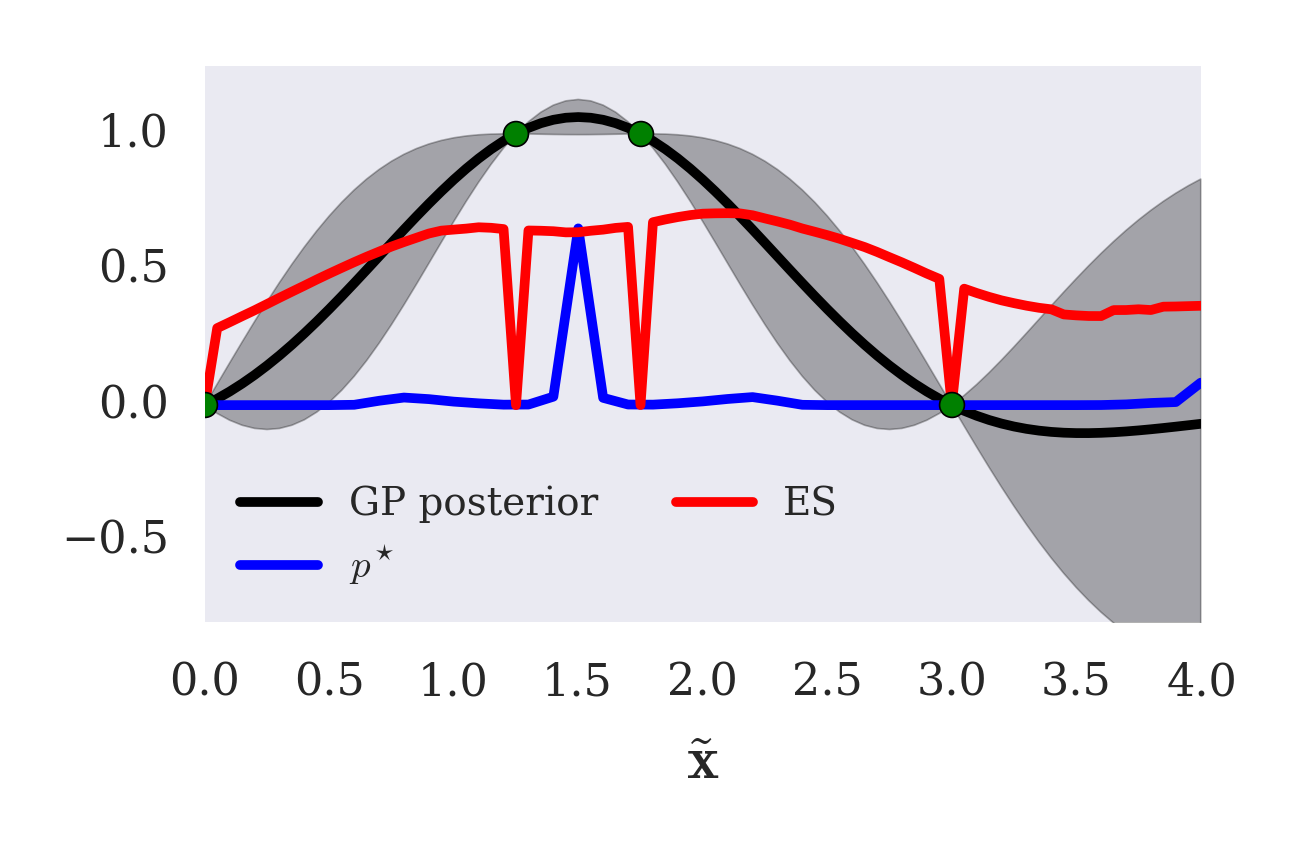
\includegraphics[width=0.48\columnwidth]{../pics/regret_illustration_3}
   \visible<3->{
     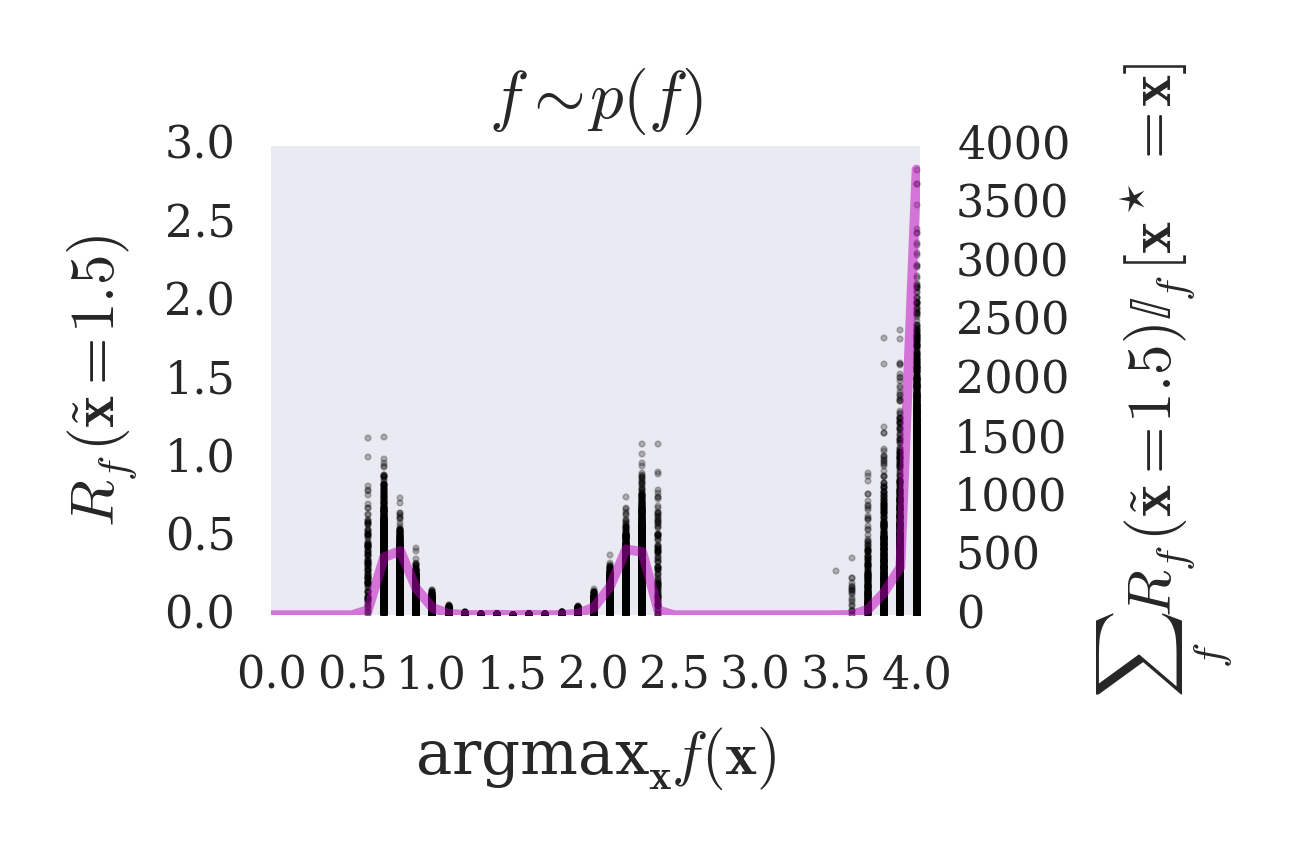
\includegraphics[width=0.48\columnwidth]{../pics/regret_scatter}
   }
   \vspace*{-.25cm}
   %\caption{\tiny (Left) GP posterior, probability of maximum $p^\star$, and expected regret ER. \visible<3->{(Right) Scatter plot of  position of optimum and regret of $\mathbf{\tilde x} = 1.5$ versus optimum in sample functions.}}
   \label{fig:MRS_illustration}
   \end{figure}
\end{frame}


\begin{frame}{Minimum Regret Search (MRS)}

Acquisition function based on minimizing the expected simple regret
\begin{itemize}
 \item Expected simple regret: $\text{ER}(p)(\mathbf{x}) = \mathbb{E}_{p(f)}[R_f(\mathbf{x})]
= \mathbb{E}_{p(f)}[\max_{\mathbf{x}} f(\mathbf{x}) - f(\mathbf{
x})]$
 \only<1>{
 \item For fixed GP $p(f)$, $\mathbf{\tilde x} = \arg\min_\mathbf{x} \text{ER}(p)(\mathbf{x})$ corresponds to the maximizer of the GP mean
 }
 \only<2->{
 \item MRS aims at selecting query points s.t.\ ER is minimized also with respect to resulting $p(f)$
 \item Myopic choice: MRS$^{\text{point}}$ selects next query point s.t.\ minimum ER is reduced the most (in expectation)
  $$a_{\text{MRS}^{\text{point}}}(\mathbf{x}^q)
  = \redub{\min_{\mathbf{\tilde x}}\text{ER}(p_n)(\mathbf{\tilde x})}_{\text{current minimum ER}}
   - \redub{\mathbb{E}_{y \vert p_n(f), \mathbf{x}^q}[\min_{\mathbf{\tilde x}}  \text{ER}(p^{[\mathbf{x}^q, y]}_n)(\mathbf{\tilde x})]}_{\text{expected posterior minimum ER for query at } \mathbf{x}^q}$$
 \visible<3->{
 \item Minimizer $\arg\min_{\mathbf{\tilde x}}\text{ER}(p_n)(\mathbf{\tilde x})$ can be seen as point estimate for $\mathbf{\tilde x}_N$ 
 \item MRS additionally also accounts for uncertainty regarding $\mathbf{\tilde x}_N$: 
  $$a_{\text{MRS}}(\mathbf{x}^q)
    = \mathbb{E}_{\mathbf{\tilde x} \sim p^\star_{\mathcal{D}_n}}[\text{ER}(p_n)(\mathbf{\tilde x})] 
     - \mathbb{E}_{y \vert p_n(f), \mathbf{x}^q}[
      \mathbb{E}_{\mathbf{\tilde x} \sim p^\star_{\mathcal{D}_n \cup \{(\mathbf{x}^q, y)\}}}[
       \text{ER}(p^{[\mathbf{x}^q, y]}_n)(\mathbf{\tilde x})]]$$
  }
  }
\end{itemize}
\only<1>{
\begin{center}
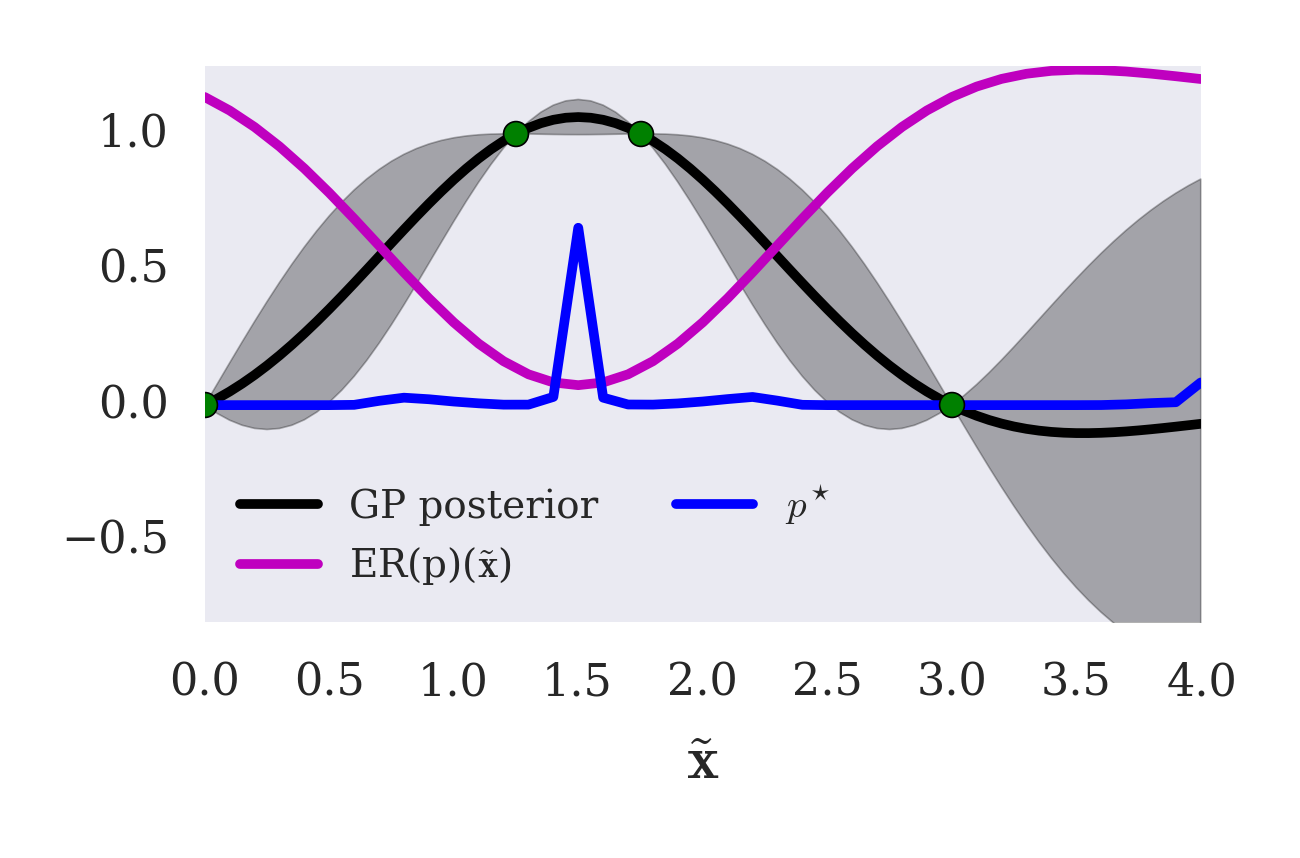
\includegraphics[width=0.58\columnwidth]{../pics/regret_illustration_4}
\end{center}
}
\end{frame}

\begin{frame}{Illustration of Acquisition Functions}
\begin{figure}
\centering
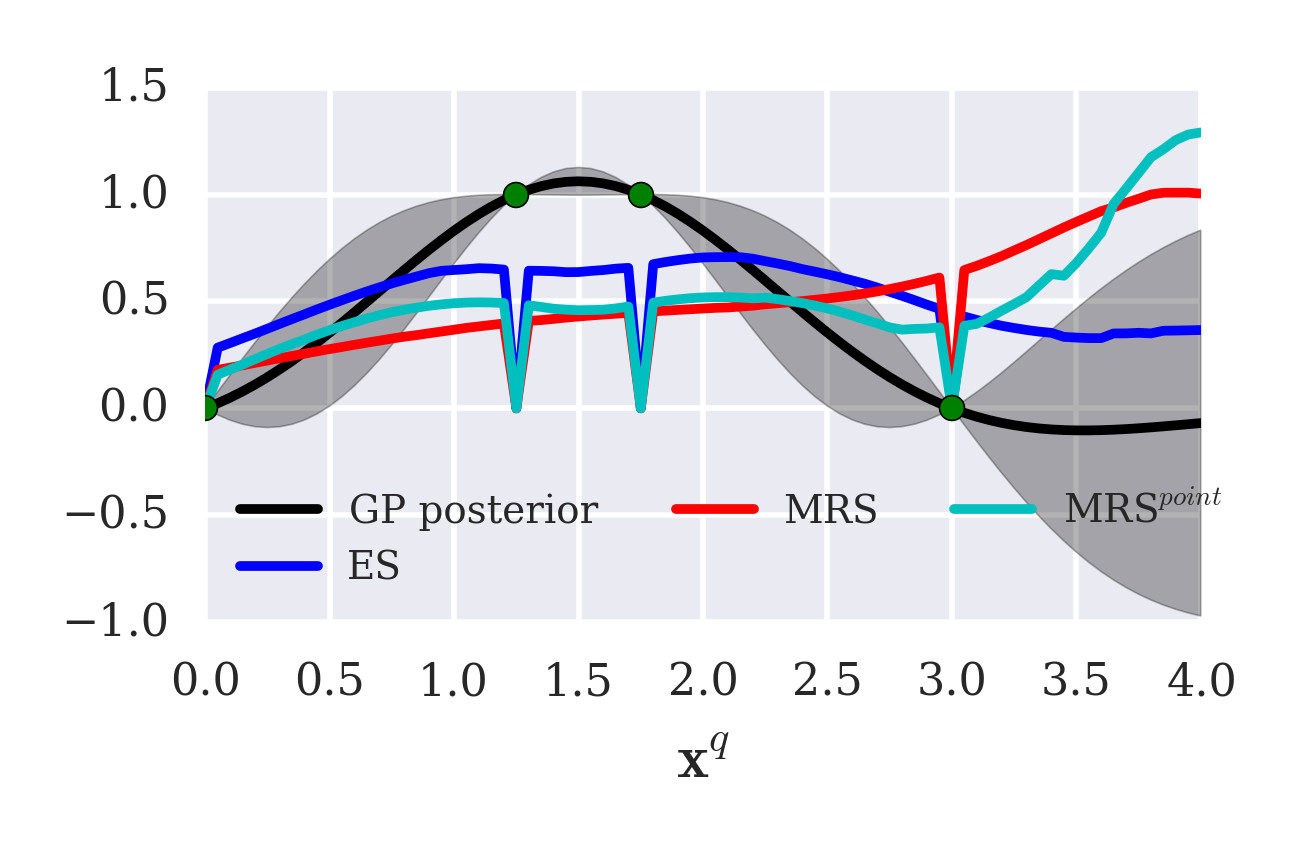
\includegraphics[width=0.48\columnwidth]{../pics/acq_comparison_2}
\end{figure}

\vspace*{-.5cm}
\begin{itemize}
\item ES tends to query close to areas where $p^\star$ is large
\item MRS$^\text{point}$ tends to query in areas which are risky for current recommendation (large simple regret possible)
\item MRS is more smooth than MRS$^\text{point}$ since it accounts for uncertainty in recommendation
\end{itemize}

\end{frame}


\begin{frame}{Experimental Setup}
Synthetic Single-Task Benchmark\footcite{hennig_entropy_2012}:
\begin{itemize}
 \item Target functions sampled from a generative model on $\mathcal{X} = [0, 1]^2$ 
 \item In practice: 
   \begin{itemize} 
   \item sample $250$ pairs $(\mathbf{x}, f(\mathbf{x}))$ from function $f \sim p(f)$
   \item fit GP to these pairs
   \item use resulting posterior mean as target function
   \end{itemize}
 \pause
 \item Gaussian noise with standard deviation $\sigma =10^{-3}$ is added to each observation
 \item Probabilistic surrogate model used in BO:\\ GP with isotropic RBF kernel of length scale $l = 0.1$ and unit signal variance
 \pause
 \item Generative model $p(f)$
    \begin{itemize} 
    \item without model mismatch: GP with isotropic RBF kernel ($l = 0.1$ and unit signal variance)
    \item with model mismatch:  GP with isotropic rational quadratic kernel ($l = 0.1$, $\alpha=1.0$ and unit signal variance)
    \end{itemize}
\end{itemize}
\end{frame}


\begin{frame}{Results: No model-mismatch}
\begin{figure}
\centering
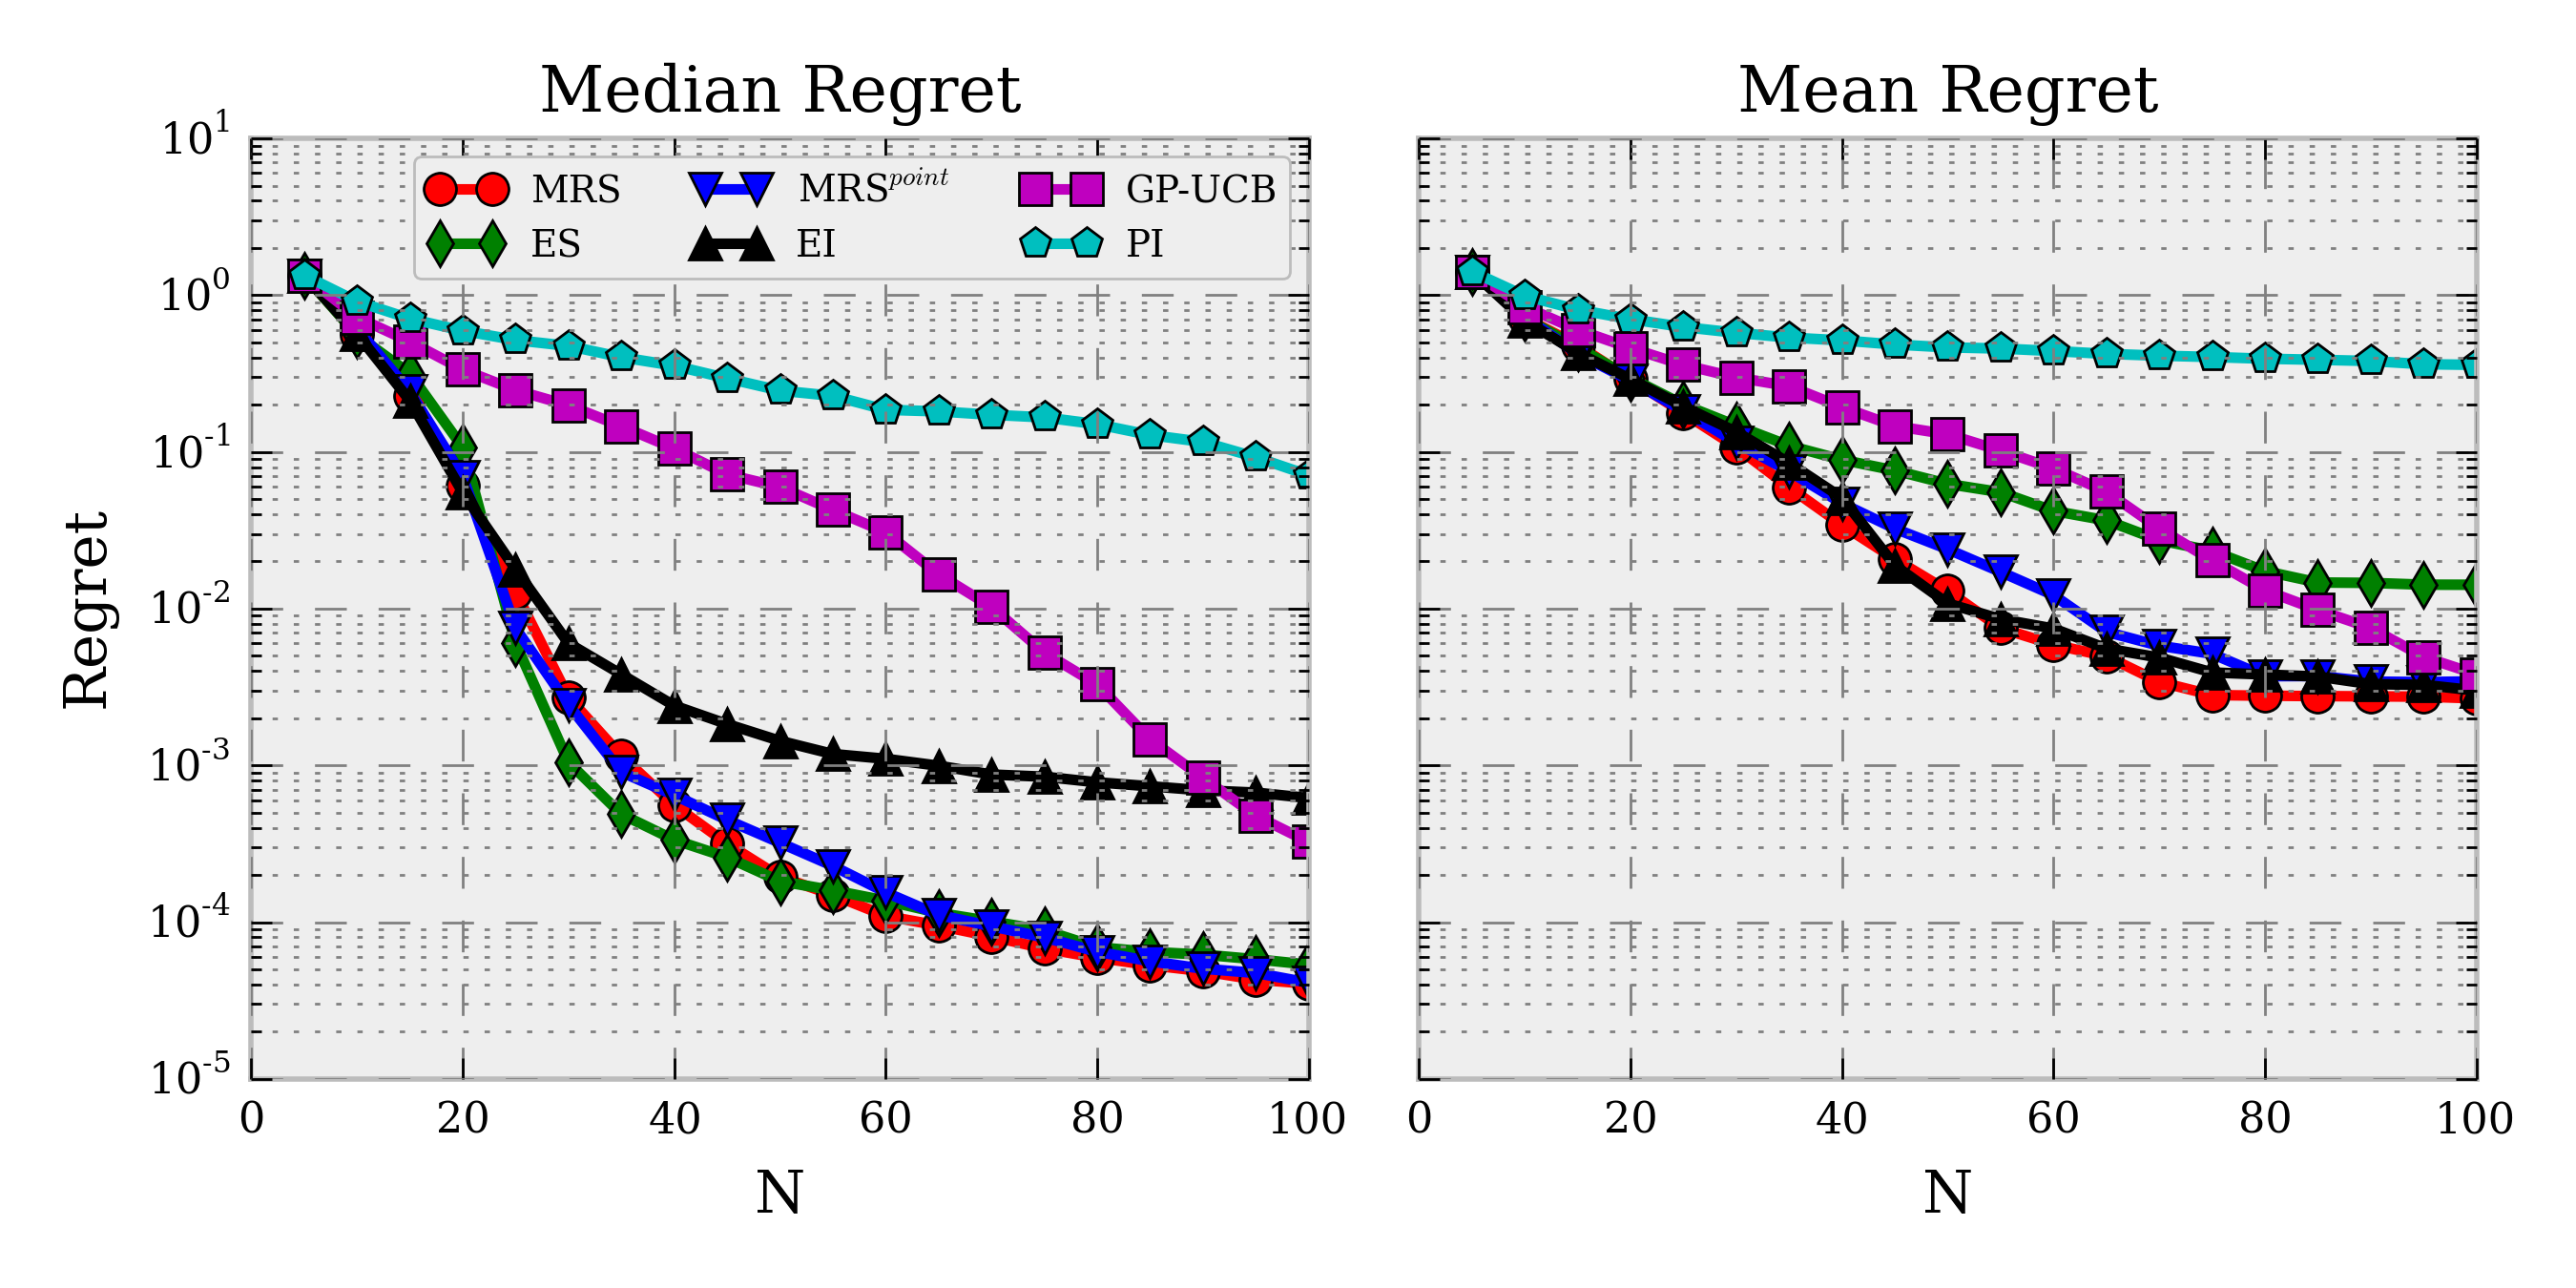
\includegraphics[width=.7\columnwidth]{../pics/empirical_comparison} \\
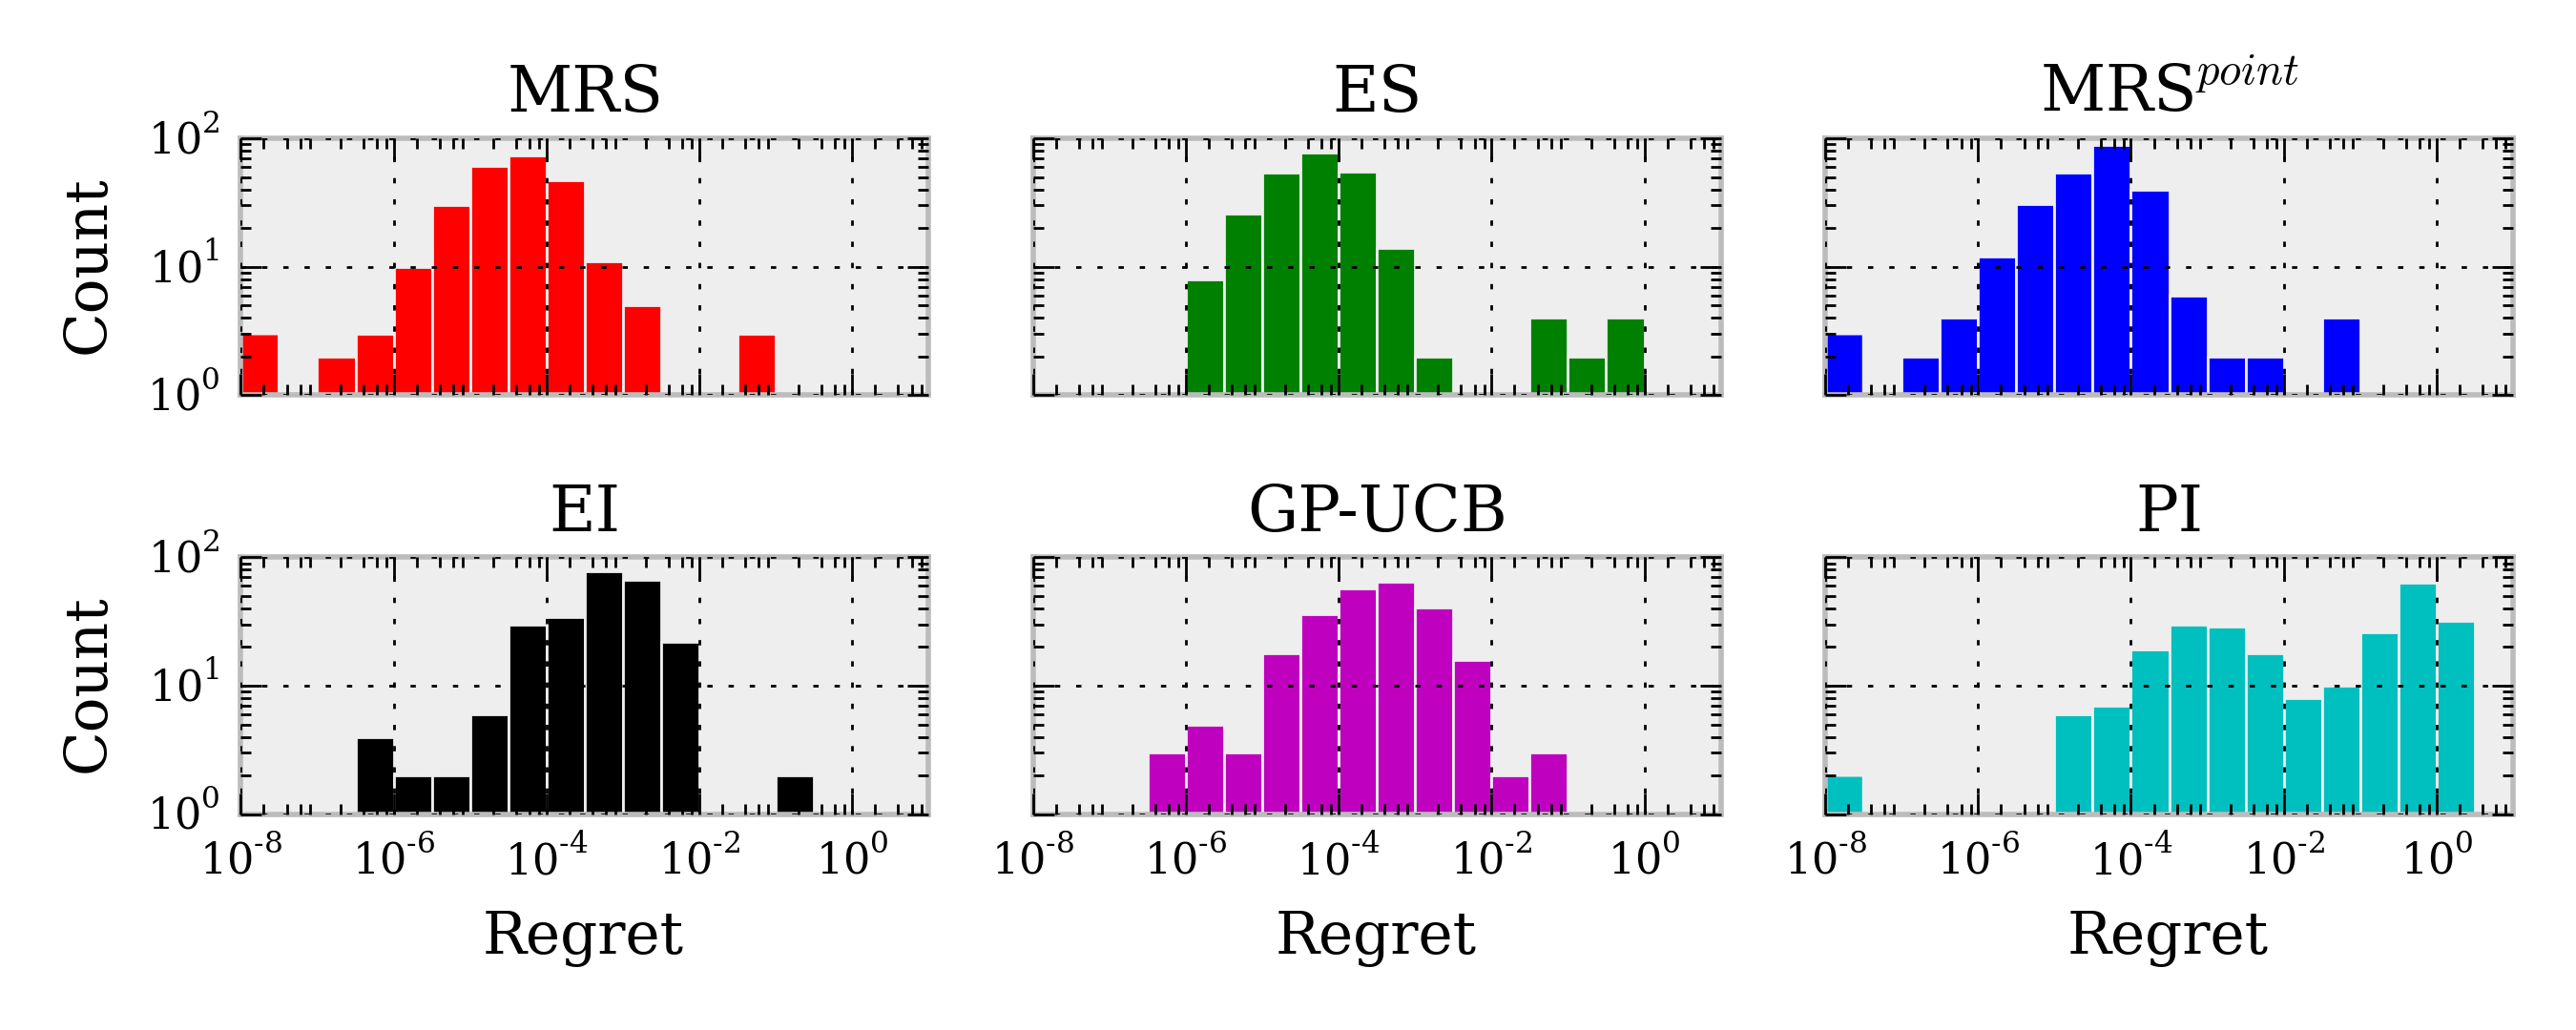
\includegraphics[width=.7\columnwidth]{../pics/hist}
\end{figure}
\end{frame}



\begin{frame}{Results: Model-mismatch}
\begin{figure}
\centering
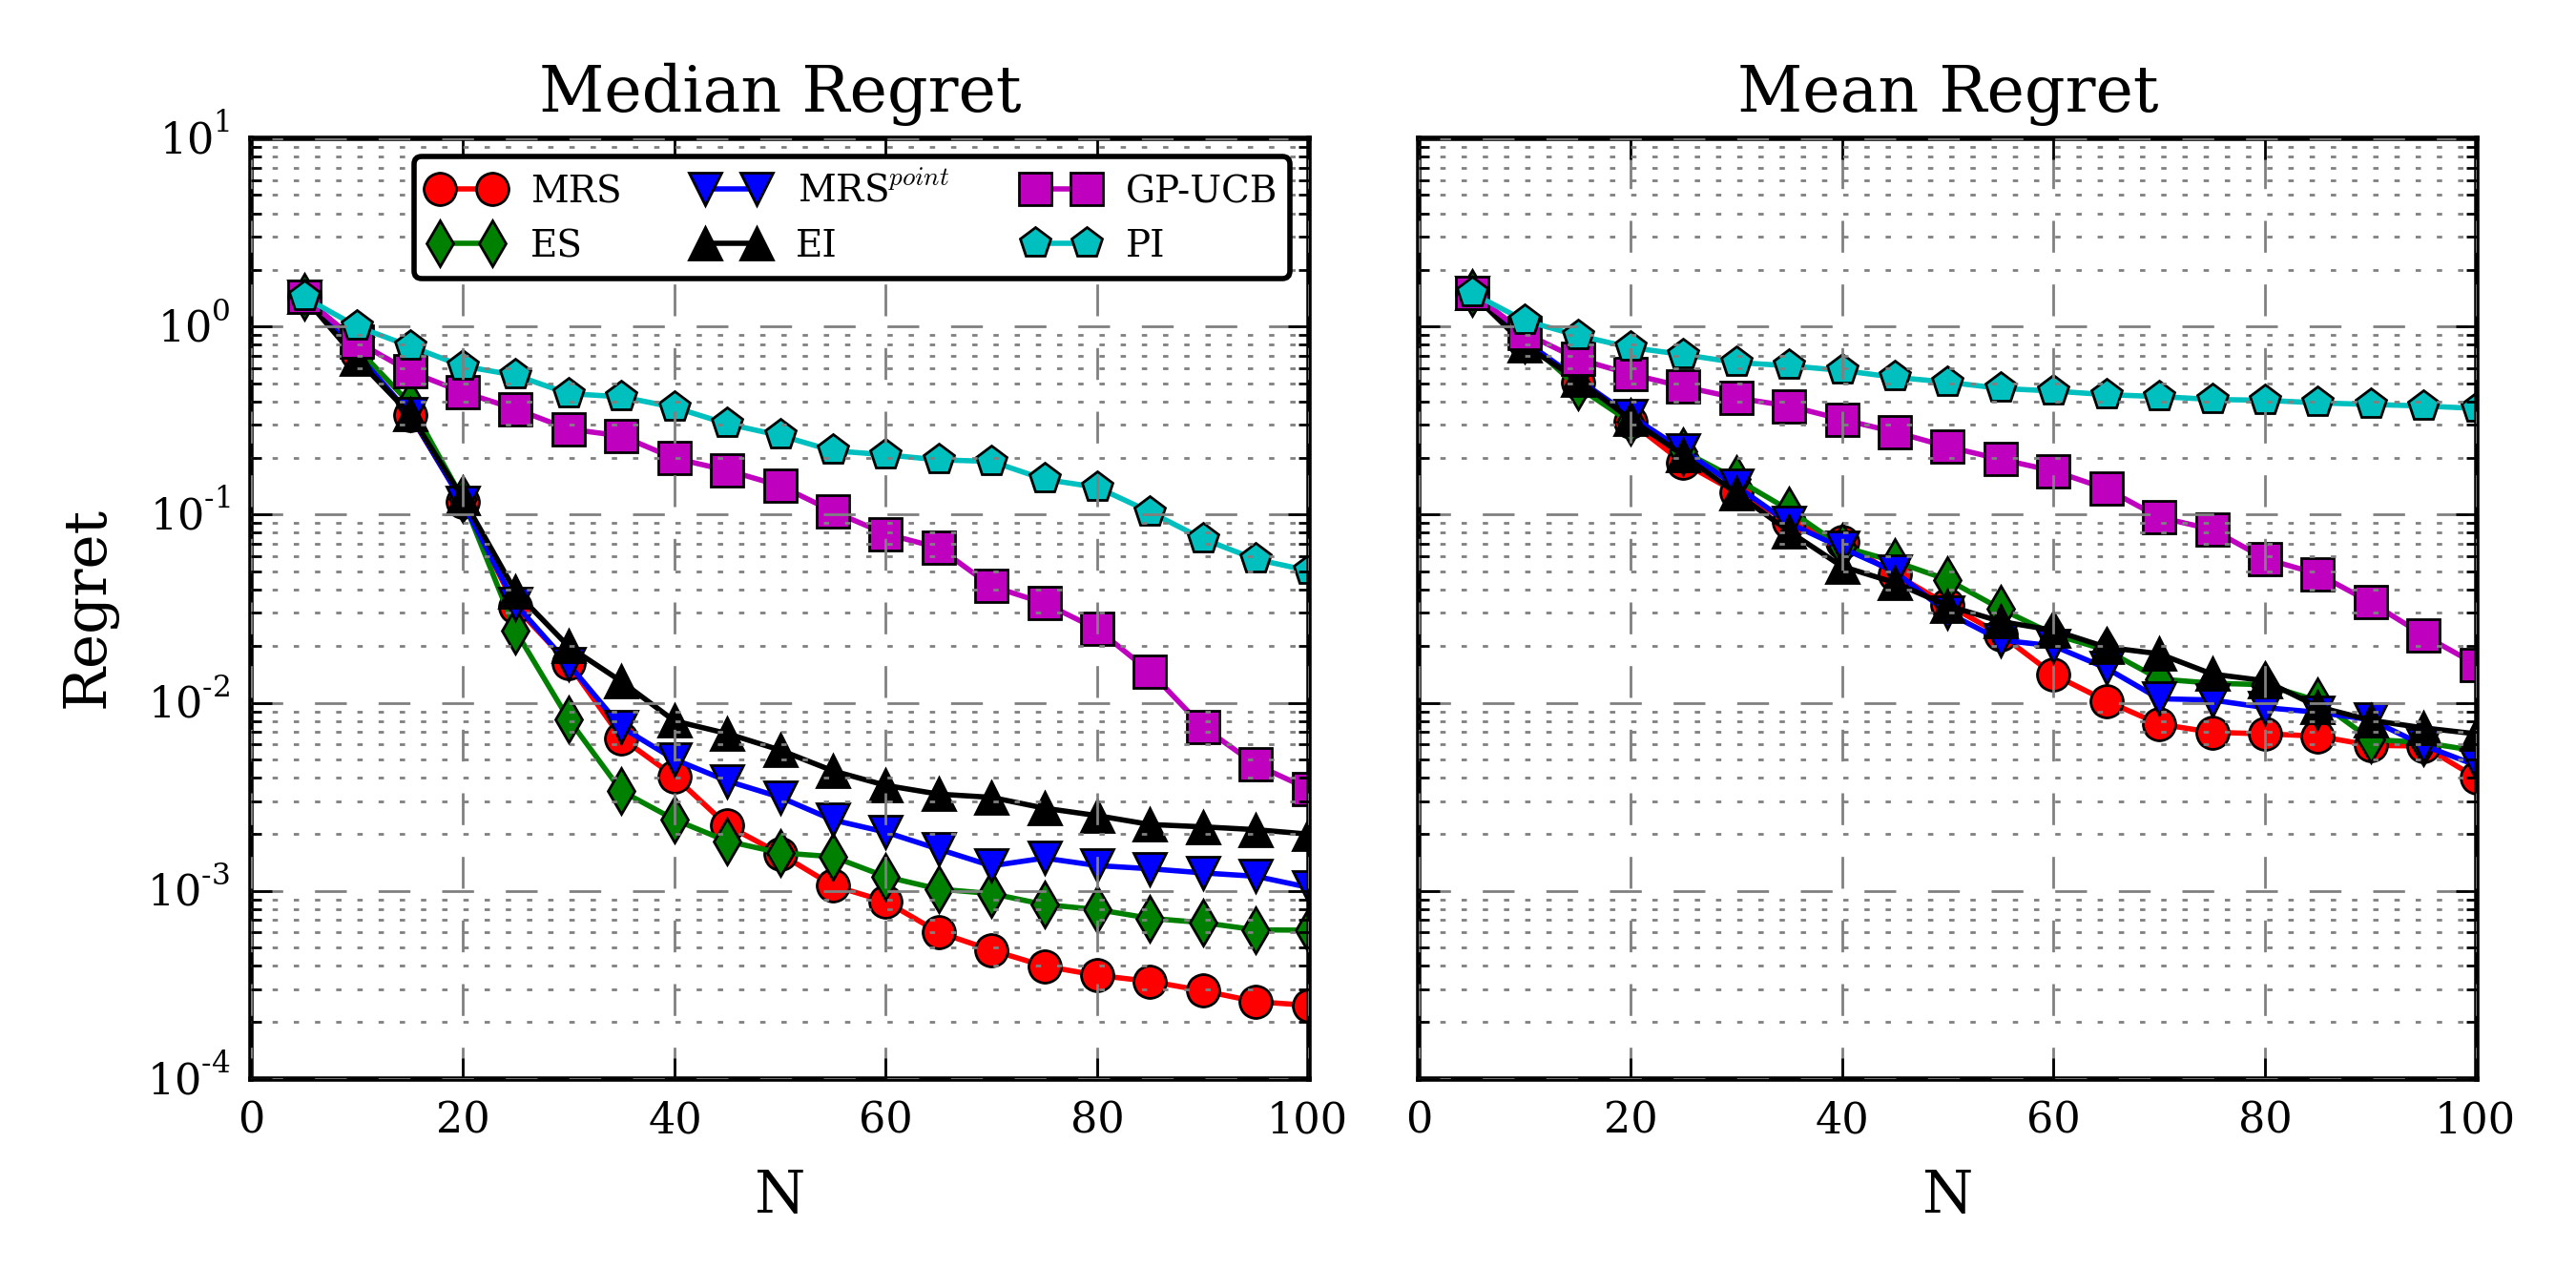
\includegraphics[width=.7\textwidth]{../pics/empirical_comparison_mm} \\
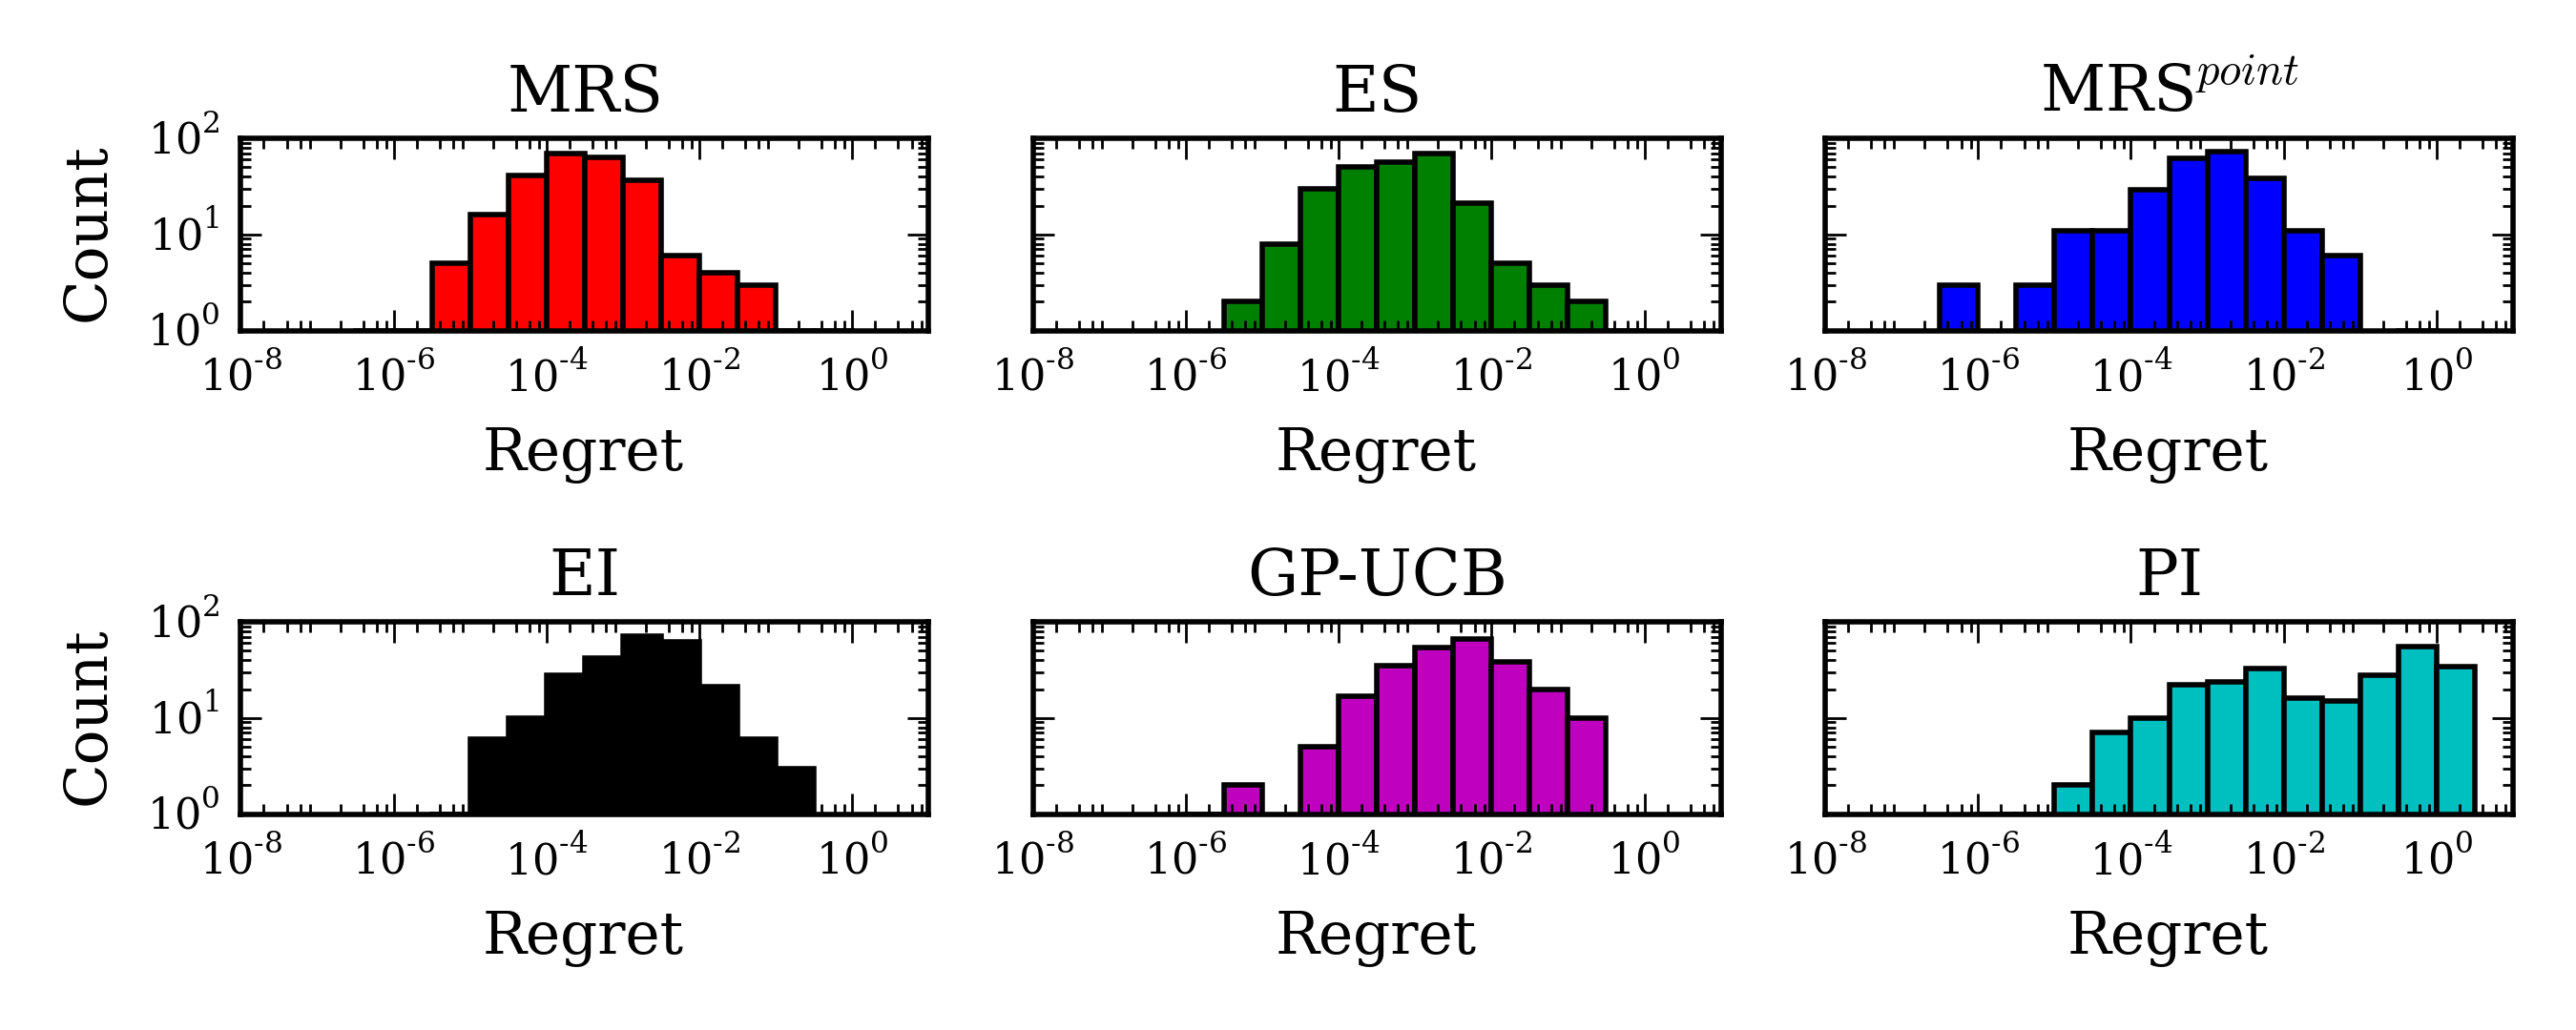
\includegraphics[width=.7\textwidth]{../pics/hist_mm}
\end{figure}
\end{frame}


\begin{frame}{Summary and Outlook}
  
  \begin{itemize}
    \item Contribution: Novel acquisition function which explicitly aims at minimizing the expected simple regret
    \pause
    \item Additional content of the paper:
    \begin{itemize}
      \item multi-task minimum regret search
      \item results on simulated robotic task
    \end{itemize}
    \pause
    \item Future work:
    \begin{itemize}
      \item treatment of GP hyperparameters
      \item more efficient approximation techniques for MRS
    \end{itemize}
    \pause
    \item Source code available at: \url{https://github.com/jmetzen/bayesian_optimization}
  \end{itemize}

  \vspace*{1cm}
  \pause
  \begin{center}
   Thank you for your attention and see you at the poster! \\
   Do you have questions, comments, or ideas?
   \end{center}

\end{frame}

\appendix

\begin{frame}[noframenumbering]{Results: MRS versus ES}
\begin{figure}
\centering
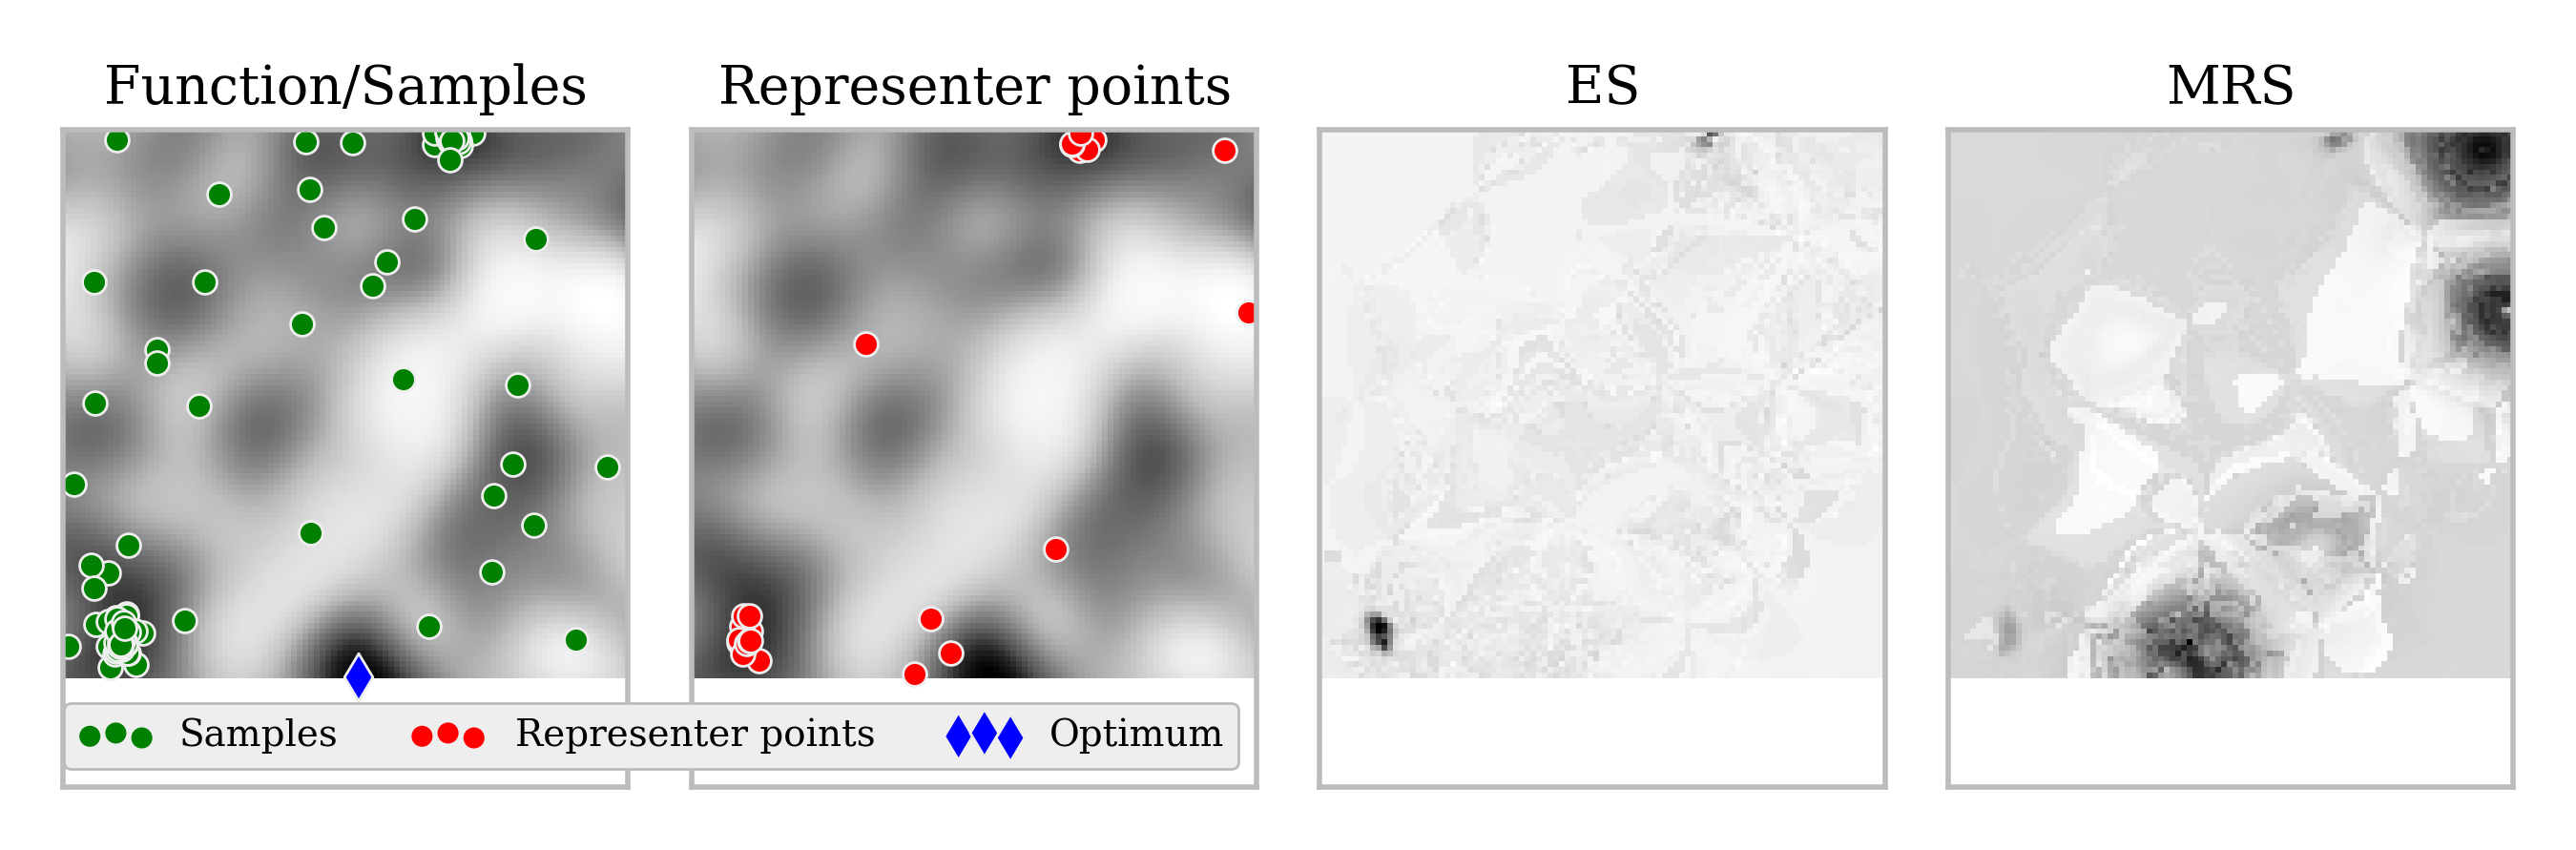
\includegraphics[width=.8\textwidth]{../pics/es_analysis}
\label{fig:es_analysis}
\end{figure}

Acquisition functions on a target function at $N=100$ and 25 representer points; darker areas correspond to larger values. ES focuses on sampling in areas with high density of $p^\star$ (many representer points), while MRS focuses on unexplored areas that are populated by representer points (non-zero $p^\star$).

\end{frame}

\end{document}
